\documentclass[11pt]{article}
\usepackage[a4paper,margin=20mm,headsep=6mm]{geometry}
\usepackage{amsmath,amssymb}
\usepackage[T1]{fontenc}
\usepackage{lmodern}
\usepackage{xcolor}
\usepackage{tikz}
\usetikzlibrary{arrows.meta}
\usepackage[most]{tcolorbox}
\usepackage{enumitem}
\usepackage{fancyhdr}
\usepackage{needspace}
\usepackage{lastpage}
\definecolor{chalk}{HTML}{2F6F8F}
\definecolor{chalkdk}{HTML}{24576F}
\definecolor{amber}{HTML}{D98A3D}
\definecolor{ink}{HTML}{1A2B34}
\definecolor{inksoft}{HTML}{4A5F68}
\definecolor{paper}{HTML}{F6F4EF}
\definecolor{line}{HTML}{DFE3E0}
\color{ink}
\setlength{\parindent}{0pt}
\setlength{\parskip}{4pt}
\pagestyle{fancy}
\fancyhf{}
\renewcommand{\headrulewidth}{0.4pt}
\renewcommand{\headrule}{\hbox to\headwidth{\color{line}\leaders\hrule height 0.4pt\hfill}}
\lhead{\small\color{inksoft}\textsc{Chapter 6 : Trigonometry}}
\rhead{\small\color{inksoft}Year 10 Methods : Question Booklet}
\cfoot{\small\color{inksoft}Page \thepage\ of \pageref{LastPage}}
\newcommand{\sectionband}[3]{%
  \needspace{5\baselineskip}\vspace{6pt}
  \begin{tcolorbox}[enhanced,colback=chalk,colframe=chalk,boxrule=0pt,left=12pt,right=12pt,top=8pt,bottom=8pt,arc=4pt,
      overlay={\node[anchor=east,text=white,opacity=0.9] at ([xshift=-12pt]frame.east) {\small\textsf{#3}};}]
    {\color{white}\large\bfseries\textsf{#1}\quad #2}
  \end{tcolorbox}}
\newtcolorbox{refbox}{enhanced,breakable,colback=paper,colframe=line,boxrule=0.6pt,left=12pt,right=12pt,top=8pt,bottom=8pt,arc=3pt}
\newtcolorbox{workedbox}{enhanced,breakable,colback=chalk!6,colframe=chalk!55,boxrule=0.7pt,left=12pt,right=12pt,top=8pt,bottom=8pt,arc=3pt,borderline west={3pt}{0pt}{chalk}}
\newcommand{\worklines}[1]{\par\vspace{2pt}\foreach \n in {1,...,#1}{\vspace{9pt}\noindent\textcolor{line!140!white}{\rule{\linewidth}{0.3pt}}\par}\vspace{2pt}}
\tikzset{figstyle/.style={line join=round,>=Stealth}}
% ---- Figure macros (schematic, not to scale) ----
% Right triangle: right angle bottom-right, angle at bottom-left.
% #1 angle label, #2 adjacent(bottom), #3 opposite(right), #4 hypotenuse
\newcommand{\figRT}[4]{\begin{center}\begin{tikzpicture}[figstyle,scale=0.8]
  \coordinate(A)at(0,0);\coordinate(B)at(3.2,0);\coordinate(C)at(3.2,2.0);
  \draw[chalkdk,very thick](A)--(B)--(C)--cycle;
  \draw[chalkdk](2.95,0)--(2.95,0.25)--(3.2,0.25);
  \draw[chalkdk](0.65,0) arc(0:32:0.65);
  \node[font=\small]at(1.0,0.2){#1};
  \node[font=\small]at(1.6,-0.32){#2};
  \node[font=\small]at(3.55,1.0){#3};
  \node[font=\small]at(1.35,1.32){#4};
\end{tikzpicture}\end{center}}
% Depression: horizontal at top-left, sight line to bottom-right.
% #1 angle, #2 vertical(height), #3 base, #4 hypotenuse
\newcommand{\figDep}[4]{\begin{center}\begin{tikzpicture}[figstyle,scale=0.8]
  \coordinate(F)at(0,0);\coordinate(T)at(0,2.0);\coordinate(P)at(3.4,0);
  \draw[chalkdk,very thick](T)--(F)--(P)--(T);
  \draw[chalkdk,dashed](T)--(1.9,2.0);
  \draw[chalkdk](0,0.25)--(0.25,0.25)--(0.25,0);
  \draw[chalkdk](1.0,2.0) arc(0:-31:1.0);
  \node[font=\small]at(1.28,1.72){#1};
  \node[font=\small]at(-0.34,1.0){#2};
  \node[font=\small]at(1.7,-0.32){#3};
  \node[font=\small]at(1.95,1.18){#4};
\end{tikzpicture}\end{center}}
% Bearing: compass + travel line. #1 math-angle, #2 bearing label, #3 distance label
\newcommand{\figBearing}[3]{\begin{center}\begin{tikzpicture}[figstyle,scale=0.8]
  \draw[chalkdk!45](0,-1.5)--(0,1.5);\draw[chalkdk!45](-1.5,0)--(1.5,0);
  \draw[chalkdk!55,->](0,0)--(0,1.75)node[above,font=\scriptsize]{N};
  \draw[chalkdk!55,->](0,0)--(1.75,0)node[right,font=\scriptsize]{E};
  \draw[chalkdk,very thick,->](0,0)--(#1:2.6);
  \draw[amber,thick](90:0.85) arc(90:#1:0.85);
  \node[font=\small,chalkdk]at({(90+#1)/2}:1.22){#2};
  \node[font=\small]at(#1:2.05)[above=1pt]{#3};
\end{tikzpicture}\end{center}}
% 8-point compass
\newcommand{\figCompass}{\begin{center}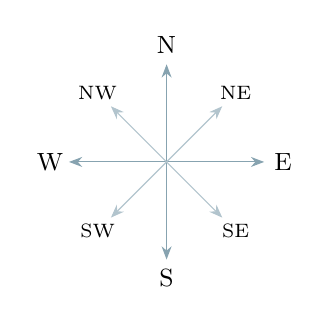
\begin{tikzpicture}[figstyle,scale=0.8]
  \foreach \a/\l in {90/N,0/E,270/S,180/W}{\draw[chalkdk!55,->](0,0)--(\a:1.55);\node[font=\small]at(\a:1.85){\l};}
  \foreach \a/\l in {45/NE,135/NW,225/SW,315/SE}{\draw[chalkdk!35,->](0,0)--(\a:1.25);\node[font=\scriptsize]at(\a:1.55){\l};}
\end{tikzpicture}\end{center}}
% General triangle. #1 vA #2 vB #3 vC #4 AB #5 BC #6 CA #7 angA #8 angB #9 angC
\newcommand{\figTri}[9]{\begin{center}\begin{tikzpicture}[figstyle,scale=0.8]
  \coordinate(A)at(0,0);\coordinate(B)at(4,0);\coordinate(C)at(1.5,2.4);
  \draw[chalkdk,very thick](A)--(B)--(C)--cycle;
  \draw[chalkdk](A)++(0:0.5) arc(0:58:0.5);
  \draw[chalkdk](B)++(136:0.5) arc(136:180:0.5);
  \draw[chalkdk](C)++(238:0.5) arc(238:316:0.5);
  \node[font=\small\bfseries,chalkdk]at(-0.24,-0.18){#1};
  \node[font=\small\bfseries,chalkdk]at(4.24,-0.18){#2};
  \node[font=\small\bfseries,chalkdk]at(1.5,2.64){#3};
  \node[font=\small]at(2,-0.3){#4};
  \node[font=\small]at(3.08,1.36){#5};
  \node[font=\small]at(0.48,1.36){#6};
  \node[font=\small]at(0.73,0.42){#7};
  \node[font=\small]at(3.2,0.36){#8};
  \node[font=\small]at(1.58,1.58){#9};
\end{tikzpicture}\end{center}}
% Rectangular prism with space diagonal. #1 length #2 depth #3 height
\newcommand{\figPrism}[3]{\begin{center}\begin{tikzpicture}[figstyle,scale=0.8]
  \coordinate(a)at(0,0);\coordinate(b)at(3,0);\coordinate(c)at(3,1.8);\coordinate(d)at(0,1.8);
  \coordinate(a2)at(1,0.7);\coordinate(b2)at(4,0.7);\coordinate(c2)at(4,2.5);\coordinate(d2)at(1,2.5);
  \draw[chalkdk,very thick](a)--(b)--(c)--(d)--cycle;
  \draw[chalkdk,very thick](b)--(b2)--(c2)--(c);
  \draw[chalkdk,very thick](d)--(d2)--(c2);
  \draw[chalkdk,dashed](a)--(a2)--(b2);\draw[chalkdk,dashed](a2)--(d2);
  \draw[amber,very thick,->](a)--(c2);
  \node[font=\small]at(1.5,-0.3){#1};
  \node[font=\small]at(3.75,0.26){#2};
  \node[font=\small]at(3.2,0.9){#3};
\end{tikzpicture}\end{center}}
% Square pyramid. #1 base side #2 height
\newcommand{\figPyramid}[2]{\begin{center}\begin{tikzpicture}[figstyle,scale=0.8]
  \coordinate(a)at(0,0);\coordinate(b)at(3,0);\coordinate(c)at(3.8,0.9);\coordinate(d)at(0.8,0.9);
  \coordinate(E)at(1.9,2.85);\coordinate(O)at(1.9,0.45);
  \draw[chalkdk,dashed](d)--(a)--(b);\draw[chalkdk,very thick](b)--(c)--(d);
  \draw[chalkdk,very thick](a)--(E)--(b);\draw[chalkdk,very thick](c)--(E);\draw[chalkdk,dashed](d)--(E);
  \draw[amber,dashed](O)--(E);
  \node[font=\small]at(1.5,-0.32){#1};
  \node[font=\small]at(2.12,1.6){#2};
\end{tikzpicture}\end{center}}
% Unit circle with radius to angle. #1 angle (deg) #2 point label
\newcommand{\figUnit}[2]{\begin{center}\begin{tikzpicture}[figstyle,scale=1.0]
  \draw[chalkdk!50,->](-1.7,0)--(1.7,0)node[right,font=\scriptsize]{$x$};
  \draw[chalkdk!50,->](0,-1.7)--(0,1.7)node[above,font=\scriptsize]{$y$};
  \draw[chalkdk,thick](0,0)circle(1.4);
  \draw[amber,very thick,->](0,0)--(#1:1.4);
  \fill[amber](#1:1.4)circle(1.7pt);
  \node[font=\scriptsize,chalkdk]at(#1:1.68){#2};
  \draw[amber](0.5,0) arc(0:#1:0.5);
\end{tikzpicture}\end{center}}
% Sine curve
\newcommand{\figSine}{\begin{center}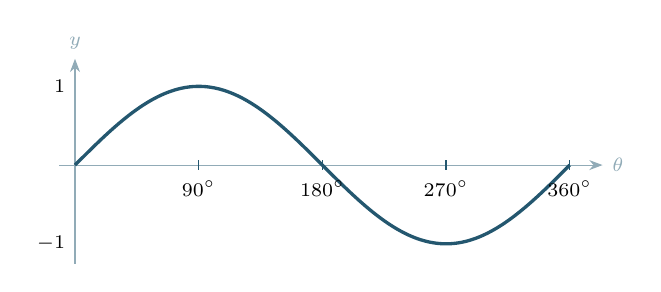
\begin{tikzpicture}[figstyle,scale=1.0]
  \draw[chalkdk!50,->](-0.2,0)--(6.7,0)node[right,font=\scriptsize]{$\theta$};
  \draw[chalkdk!50,->](0,-1.25)--(0,1.35)node[above,font=\scriptsize]{$y$};
  \draw[chalkdk,very thick,domain=0:6.283,samples=90,smooth]plot(\x,{sin(\x r)});
  \foreach \x/\l in {1.571/90,3.1416/180,4.712/270,6.283/360}{\draw[chalkdk](\x,-0.06)--(\x,0.06);\node[font=\scriptsize,below]at(\x,-0.08){$\l^\circ$};}
  \node[font=\scriptsize,left]at(0,1){$1$};\node[font=\scriptsize,left]at(0,-1){$-1$};
\end{tikzpicture}\end{center}}
% Cosine curve
\newcommand{\figCos}{\begin{center}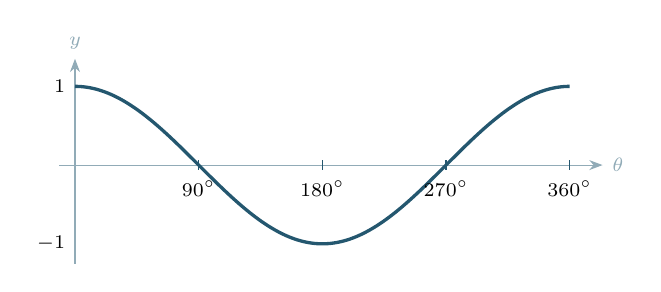
\begin{tikzpicture}[figstyle,scale=1.0]
  \draw[chalkdk!50,->](-0.2,0)--(6.7,0)node[right,font=\scriptsize]{$\theta$};
  \draw[chalkdk!50,->](0,-1.25)--(0,1.35)node[above,font=\scriptsize]{$y$};
  \draw[chalkdk,very thick,domain=0:6.283,samples=90,smooth]plot(\x,{cos(\x r)});
  \foreach \x/\l in {1.571/90,3.1416/180,4.712/270,6.283/360}{\draw[chalkdk](\x,-0.06)--(\x,0.06);\node[font=\scriptsize,below]at(\x,-0.08){$\l^\circ$};}
  \node[font=\scriptsize,left]at(0,1){$1$};\node[font=\scriptsize,left]at(0,-1){$-1$};
\end{tikzpicture}\end{center}}
% Two special triangles
\newcommand{\figSpecials}{\begin{center}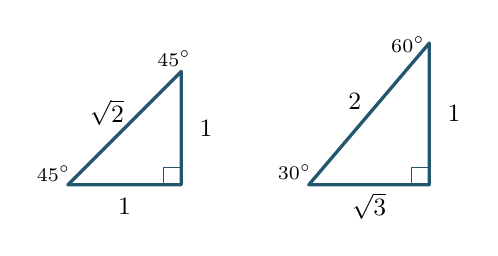
\begin{tikzpicture}[figstyle,scale=0.9,font=\small]
  \draw[chalkdk,very thick](0,0)--(1.6,0)--(1.6,1.6)--cycle;
  \draw[chalkdk](1.35,0)--(1.35,0.25)--(1.6,0.25);
  \node at(0.8,-0.3){$1$};\node at(1.95,0.8){$1$};\node at(0.55,1.02){$\sqrt2$};
  \node[font=\scriptsize]at(-.20,0.16){$45^\circ$};\node[font=\scriptsize]at(1.5,1.78){$45^\circ$};
  \begin{scope}[xshift=3.4cm]
   \draw[chalkdk,very thick](0,0)--(1.7,0)--(1.7,2.0)--cycle;
   \draw[chalkdk](1.45,0)--(1.45,0.25)--(1.7,0.25);
   \node at(0.85,-0.3){$\sqrt3$};\node at(2.05,1.0){$1$};\node at(0.65,1.18){$2$};
   \node[font=\scriptsize]at(-0.2,0.18){$30^\circ$};\node[font=\scriptsize]at(1.4,1.98){$60^\circ$};
  \end{scope}
\end{tikzpicture}\end{center}}
% Graph grid (blank, for sketching)
\newcommand{\graphgrid}{\par\vspace{4pt}\begin{center}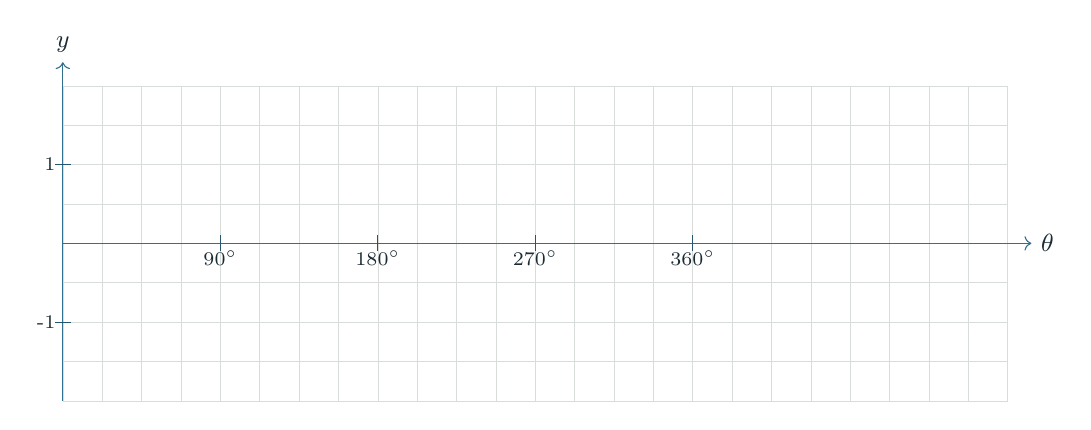
\begin{tikzpicture}[scale=1]
    \draw[step=0.5cm,line!120!white,very thin](0,0) grid (12,4);
    \draw[chalk,->](0,2)--(12.3,2)node[right,ink]{\small $\theta$};
    \draw[chalk,->](0,0)--(0,4.3)node[above,ink]{\small $y$};
    \foreach \x/\lab in {2/90,4/180,6/270,8/360}{\draw[chalkdk](\x,1.9)--(\x,2.1)node[below=2pt,ink]{\scriptsize $\lab^\circ$};}
    \draw[chalkdk](-0.1,3)--(0.1,3)node[left=2pt,ink]{\scriptsize 1};
    \draw[chalkdk](-0.1,1)--(0.1,1)node[left=2pt,ink]{\scriptsize -1};
  \end{tikzpicture}\end{center}}
\begin{document}
\thispagestyle{empty}
\begin{tikzpicture}[remember picture,overlay]
  \fill[chalk] (current page.north west) rectangle ([yshift=-62mm]current page.north east);
  \node[anchor=north west,text=white,align=left] at ([xshift=20mm,yshift=-20mm]current page.north west)
    {{\Huge\bfseries\textsf{Chapter 6: Trigonometry}}\\[4mm]{\LARGE\textsf{Student Question Booklet}}\\[3mm]{\large\textsf{Year 10 Mathematical Methods : 2026}}};
\end{tikzpicture}
\vspace{58mm}

\vspace{6mm}
\begin{refbox}
{\bfseries\color{chalkdk}How to use this booklet}\\[2pt]
This booklet is your \textbf{map through Chapter 6}. For every section you will find:
\begin{itemize}[leftmargin=16pt,itemsep=2pt,topsep=3pt]
  \item \textbf{Worked examples} --- fully solved examples with a labelled diagram, plus the matching textbook example numbers and pages to cross-reference.
  \item \textbf{Question sets} --- the questions to practise, grouped by \textit{Building Understanding}, \textit{Fluency}, \textit{Problem-solving}, \textit{Reasoning} and \textit{Enrichment}, with page numbers. Find them in your own textbook.
  \item \textbf{Hurdle questions} --- five questions you \textbf{must} be able to do to pass the section, each with a diagram and working space.
\end{itemize}
\vspace{2pt}{\small\color{inksoft}Diagrams are schematic (not to scale). Sections marked \textsf{10A} are extension. Keep your calculator in \textbf{DEGREE} mode; round as instructed and always show working.}
\end{refbox}
\vspace{4mm}{\small\color{inksoft}Page references are to \emph{Essential Mathematics for the Victorian Curriculum 10 \& 10A}, 3rd ed. Question sets belong to the textbook; the worked examples, diagrams and hurdle questions are original material written for this course.}
\clearpage
\newpage
\quad
\clearpage

\sectionband{6A}{Trigonometric ratios}{CORE}

\begin{refbox}
{\bfseries\color{chalkdk}Textbook worked examples}\;\textcolor{inksoft}{\small(cross-reference in your textbook)}\\[3pt]
\begin{itemize}[leftmargin=16pt,itemsep=1pt,topsep=2pt]
  \item \textbf{Example 1} --- Solving for an unknown in the numerator \textcolor{inksoft}{(p.\,496)}
  \item \textbf{Example 2} --- Solving for an unknown in the denominator \textcolor{inksoft}{(p.\,497)}
\end{itemize}
\vspace{4pt}{\bfseries\color{chalkdk}Question sets}\;\textcolor{inksoft}{\small(practise from your textbook)}\\[3pt]
\begin{itemize}[leftmargin=16pt,itemsep=1pt,topsep=2pt]
  \item \textbf{Building Understanding:} Q1--3 \textcolor{inksoft}{(p.\,495)}
  \item \textbf{Fluency:} Q1--3 \textcolor{inksoft}{(p.\,498--500)}
  \item \textbf{Problem-solving:} Q4--9 \textcolor{inksoft}{(p.\,500--501)}
  \item \textbf{Reasoning:} Q10--11 \textcolor{inksoft}{(p.\,501)}
  \item \textbf{Enrichment: Exploring identities:} Q12 \textcolor{inksoft}{(p.\,501)}
\end{itemize}\end{refbox}

\vspace{4pt}{\bfseries\color{chalkdk}\large Worked examples}\;\textcolor{inksoft}{\small(study the method, then try the hurdles)}\par

\needspace{8\baselineskip}\begin{workedbox}

{\bfseries\color{chalkdk}Finding a side --- unknown in the numerator}\par\vspace{3pt}

Find $x$, correct to two decimal places. The hypotenuse is $10\text{ cm}$, the marked angle is $34^\circ$, and $x$ is the side \emph{opposite} that angle.\par\vspace{2pt}

\figRT{$34^\circ$}{}{$x$}{$10$}

{\bfseries Solution.}\ The unknown is opposite and the hypotenuse is known, so use \textbf{sine} ($\sin=\tfrac{\text{opp}}{\text{hyp}}$). \[ \sin 34^\circ=\frac{x}{10} \;\Rightarrow\; x=10\sin 34^\circ=5.59\text{ cm (2 dp).} \]

\end{workedbox}

\needspace{8\baselineskip}\begin{workedbox}

{\bfseries\color{chalkdk}Finding a side --- unknown in the denominator}\par\vspace{3pt}

Find the hypotenuse $x$, correct to two decimal places, when the side \emph{opposite} a $40^\circ$ angle is $6\text{ m}$.\par\vspace{2pt}

\figRT{$40^\circ$}{}{$6$}{$x$}

{\bfseries Solution.}\ The unknown is the hypotenuse, so it sits in the denominator. \[ \sin 40^\circ=\frac{6}{x} \;\Rightarrow\; x=\frac{6}{\sin 40^\circ}=9.33\text{ m (2 dp).} \]

\end{workedbox}
\newpage
\vspace{6pt}{\bfseries\color{amber}\large Hurdle questions --- Section 6A}\;\textcolor{inksoft}{\small(show all working)}\par\vspace{2pt}

\begin{enumerate}[leftmargin=20pt,itemsep=8pt,topsep=4pt,label=\textbf{H\arabic*.}]

\needspace{8\baselineskip}

  \item Find the value of $x$, correct to two decimal places. A right-angled triangle has a hypotenuse of $14\text{ cm}$ and the angle between the hypotenuse and the base is $37^\circ$; $x$ is the side opposite the $37^\circ$ angle.

\figRT{$37^\circ$}{}{$x$}{$14$}

  \worklines{4}

\needspace{8\baselineskip}

  \item Find the value of $x$, correct to two decimal places, where $x$ is the \emph{adjacent} side: the angle is $42^\circ$ and the opposite side is $8.5\text{ m}$. \emph{(Hint: the unknown is in the denominator.)}

\figRT{$42^\circ$}{$x$}{$8.5$}{}

  \worklines{4}

\needspace{8\baselineskip}

  \item A right-angled triangle has an angle of $28^\circ$ and the side \emph{opposite} this angle is $5.2\text{ m}$. Find the length of the hypotenuse, correct to two decimal places.

\figRT{$28^\circ$}{}{$5.2$}{$x$}

  \worklines{4}

\needspace{8\baselineskip}

  \item A skateboard ramp rises at an angle of $15^\circ$ to the horizontal over a horizontal run of $4\text{ m}$. Find the vertical height of the ramp, correct to two decimal places.

\figRT{$15^\circ$}{$4$}{$x$}{}

  \worklines{4}

\needspace{8\baselineskip}

  \item Find the length of the unknown side marked $x$: the known angle is $60^\circ$, the side adjacent to it is $9\text{ cm}$, and $x$ is the side opposite the $60^\circ$ angle. Give your answer correct to two decimal places.

\figRT{$60^\circ$}{$9$}{$x$}{}

  \worklines{4}

\end{enumerate}\clearpage

\sectionband{6B}{Finding unknown angles}{CORE}

\begin{refbox}
{\bfseries\color{chalkdk}Textbook worked examples}\;\textcolor{inksoft}{\small(cross-reference in your textbook)}\\[3pt]
\begin{itemize}[leftmargin=16pt,itemsep=1pt,topsep=2pt]
  \item \textbf{Example 3} --- Finding angles \textcolor{inksoft}{(p.\,503)}
  \item \textbf{Example 4} --- Working with simple trigonometric applications \textcolor{inksoft}{(p.\,504)}
\end{itemize}
\vspace{4pt}{\bfseries\color{chalkdk}Question sets}\;\textcolor{inksoft}{\small(practise from your textbook)}\\[3pt]
\begin{itemize}[leftmargin=16pt,itemsep=1pt,topsep=2pt]
  \item \textbf{Building Understanding:} Q1--2 \textcolor{inksoft}{(p.\,503)}
  \item \textbf{Fluency:} Q1--3 \textcolor{inksoft}{(p.\,505--506)}
  \item \textbf{Problem-solving:} Q4--7 \textcolor{inksoft}{(p.\,506)}
  \item \textbf{Reasoning:} Q8--10 \textcolor{inksoft}{(p.\,506--507)}
  \item \textbf{Enrichment: A special triangle:} Q11 \textcolor{inksoft}{(p.\,507)}
\end{itemize}\end{refbox}

\vspace{4pt}{\bfseries\color{chalkdk}\large Worked examples}\;\textcolor{inksoft}{\small(study the method, then try the hurdles)}\par

\needspace{8\baselineskip}\begin{workedbox}

{\bfseries\color{chalkdk}Finding an unknown angle}\par\vspace{3pt}

Find $\theta$, correct to one decimal place, when the side opposite $\theta$ is $4$ and the hypotenuse is $9$.\par\vspace{2pt}

\figRT{$\theta$}{}{$4$}{$9$}

{\bfseries Solution.}\ Opposite and hypotenuse are known, so use the inverse sine. \[ \sin\theta=\frac{4}{9} \;\Rightarrow\; \theta=\sin^{-1}\!\left(\tfrac{4}{9}\right)=26.4^\circ\ \text{(1 dp).} \]

\end{workedbox}

\needspace{8\baselineskip}\begin{workedbox}

{\bfseries\color{chalkdk}Angle in an application}\par\vspace{3pt}

A ramp has a sloping surface $8\text{ m}$ long that reaches $1.5\text{ m}$ vertically. Find the angle the ramp makes with the horizontal, to one decimal place.\par\vspace{2pt}

\figRT{$\theta$}{}{$1.5$}{$8$}

{\bfseries Solution.}\ The $1.5\text{ m}$ rise is opposite the angle and the $8\text{ m}$ slope is the hypotenuse. \[ \sin\theta=\frac{1.5}{8} \;\Rightarrow\; \theta=\sin^{-1}(0.1875)=10.8^\circ\ \text{(1 dp).} \]

\end{workedbox}
\newpage
\vspace{6pt}{\bfseries\color{amber}\large Hurdle questions --- Section 6B}\;\textcolor{inksoft}{\small(show all working)}\par\vspace{2pt}

\begin{enumerate}[leftmargin=20pt,itemsep=8pt,topsep=4pt,label=\textbf{H\arabic*.}]

\needspace{8\baselineskip}

  \item Find the angle $\theta$, correct to one decimal place, in a right-angled triangle where the side opposite $\theta$ is $7$ and the hypotenuse is $11$.

\figRT{$\theta$}{}{$7$}{$11$}

  \worklines{4}

\needspace{8\baselineskip}

  \item Find the angle $\theta$, correct to one decimal place, in a right-angled triangle where the side opposite $\theta$ is $5$ and the adjacent side is $9$.

\figRT{$\theta$}{$9$}{$5$}{}

  \worklines{4}

\needspace{8\baselineskip}

  \item A $6\text{ m}$ ladder leans against a wall, reaching $5.2\text{ m}$ up the wall. Find the angle the ladder makes with the ground, correct to one decimal place.

\figRT{$\theta$}{}{$5.2$}{$6$}

  \worklines{4}

\needspace{8\baselineskip}

  \item A right-angled triangle has the two shorter sides (legs) of length $8$ and $15$. Find the sizes of \emph{both} non-right angles, correct to one decimal place.

\figRT{$\alpha$}{$15$}{$8$}{}

  \worklines{4}

\needspace{8\baselineskip}

  \item A straight road climbs $45\text{ m}$ vertically over a horizontal distance of $300\text{ m}$. Find the angle of incline of the road, correct to one decimal place.

\figRT{$\theta$}{$300$}{$45$}{}

  \worklines{4}

\end{enumerate}\clearpage

\sectionband{6C}{Applications in two dimensions}{CORE}

\begin{refbox}
{\bfseries\color{chalkdk}Textbook worked examples}\;\textcolor{inksoft}{\small(cross-reference in your textbook)}\\[3pt]
\begin{itemize}[leftmargin=16pt,itemsep=1pt,topsep=2pt]
  \item \textbf{Example 5} --- Working with an angle of elevation \textcolor{inksoft}{(p.\,509)}
  \item \textbf{Example 6} --- Working with an angle of depression \textcolor{inksoft}{(p.\,510)}
\end{itemize}
\vspace{4pt}{\bfseries\color{chalkdk}Question sets}\;\textcolor{inksoft}{\small(practise from your textbook)}\\[3pt]
\begin{itemize}[leftmargin=16pt,itemsep=1pt,topsep=2pt]
  \item \textbf{Building Understanding:} Q1--2 \textcolor{inksoft}{(p.\,509)}
  \item \textbf{Fluency:} Q1--6 \textcolor{inksoft}{(p.\,511)}
  \item \textbf{Problem-solving:} Q7--9 \textcolor{inksoft}{(p.\,511--512)}
  \item \textbf{Reasoning:} Q10--13 \textcolor{inksoft}{(p.\,512--513)}
  \item \textbf{Enrichment: Vegetable garden design:} Q14 \textcolor{inksoft}{(p.\,513)}
\end{itemize}\end{refbox}

\vspace{4pt}{\bfseries\color{chalkdk}\large Worked examples}\;\textcolor{inksoft}{\small(study the method, then try the hurdles)}\par

\needspace{8\baselineskip}\begin{workedbox}

{\bfseries\color{chalkdk}Angle of elevation}\par\vspace{3pt}

From a point $30\text{ m}$ from the base of a tower on level ground, the angle of elevation to the top is $41^\circ$. Find the height $h$, to two decimal places.\par\vspace{2pt}

\figRT{$41^\circ$}{$30$}{$h$}{}

{\bfseries Solution.}\ Height is opposite the angle and $30\text{ m}$ is adjacent, so use \textbf{tangent}. \[ \tan 41^\circ=\frac{h}{30} \;\Rightarrow\; h=30\tan 41^\circ=26.08\text{ m (2 dp).} \]

\end{workedbox}

\needspace{8\baselineskip}\begin{workedbox}

{\bfseries\color{chalkdk}Angle of depression}\par\vspace{3pt}

From the top of a $50\text{ m}$ cliff, the angle of depression to a boat is $20^\circ$. Find the horizontal distance $d$ to the boat, to two decimal places.\par\vspace{2pt}

\figDep{$20^\circ$}{$50$}{$d$}{}

{\bfseries Solution.}\ The depression angle equals the elevation angle from the boat. The $50\text{ m}$ height is opposite and $d$ is adjacent. \[ \tan 20^\circ=\frac{50}{d} \;\Rightarrow\; d=\frac{50}{\tan 20^\circ}=137.37\text{ m (2 dp).} \]

\end{workedbox}
\newpage
\vspace{6pt}{\bfseries\color{amber}\large Hurdle questions --- Section 6C}\;\textcolor{inksoft}{\small(show all working)}\par\vspace{2pt}

\begin{enumerate}[leftmargin=20pt,itemsep=8pt,topsep=4pt,label=\textbf{H\arabic*.}]

\needspace{8\baselineskip}

  \item From a point on level ground $20\text{ m}$ from the base of a tree, the angle of elevation to the top of the tree is $32^\circ$. Find the height of the tree, correct to two decimal places.

\figRT{$32^\circ$}{$20$}{$h$}{}

  \worklines{4}

\needspace{8\baselineskip}

  \item From the top of a cliff $80\text{ m}$ high, the angle of depression to a boat at sea is $24^\circ$. Find the horizontal distance from the base of the cliff to the boat, correct to two decimal places.

\figDep{$24^\circ$}{$80$}{$d$}{}

  \worklines{4}

\needspace{8\baselineskip}

  \item A kite is flying on a taut string $50\text{ m}$ long that makes an angle of $55^\circ$ with the horizontal. Find the height of the kite above the ground, correct to two decimal places.

\figRT{$55^\circ$}{}{$h$}{$50$}

  \worklines{4}

\needspace{8\baselineskip}

  \item The angle of elevation to the top of a communications tower from a point $60\text{ m}$ from its base (on level ground) is $38^\circ$. Find the height of the tower, correct to two decimal places.

\figRT{$38^\circ$}{$60$}{$h$}{}

  \worklines{4}

\needspace{8\baselineskip}

  \item From the top of a $25\text{ m}$ lighthouse, the angle of depression to a swimmer is $18^\circ$. Find the horizontal distance from the base of the lighthouse to the swimmer, correct to two decimal places.

\figDep{$18^\circ$}{$25$}{$d$}{}

  \worklines{4}

\end{enumerate}\clearpage

\sectionband{6D}{Directions and bearings}{CORE}

\begin{refbox}
{\bfseries\color{chalkdk}Textbook worked examples}\;\textcolor{inksoft}{\small(cross-reference in your textbook)}\\[3pt]
\begin{itemize}[leftmargin=16pt,itemsep=1pt,topsep=2pt]
  \item \textbf{Example 7} --- Stating a direction \textcolor{inksoft}{(p.\,515)}
  \item \textbf{Example 8} --- Using bearings with trigonometry \textcolor{inksoft}{(p.\,516)}
\end{itemize}
\vspace{4pt}{\bfseries\color{chalkdk}Question sets}\;\textcolor{inksoft}{\small(practise from your textbook)}\\[3pt]
\begin{itemize}[leftmargin=16pt,itemsep=1pt,topsep=2pt]
  \item \textbf{Building Understanding:} Q1--3 \textcolor{inksoft}{(p.\,515)}
  \item \textbf{Fluency:} Q1--7 \textcolor{inksoft}{(p.\,517--518)}
  \item \textbf{Problem-solving:} Q8--11 \textcolor{inksoft}{(p.\,518--519)}
  \item \textbf{Reasoning:} Q12--14 \textcolor{inksoft}{(p.\,519--520)}
  \item \textbf{Enrichment: Navigation challenges:} Q15--16 \textcolor{inksoft}{(p.\,520)}
\end{itemize}\end{refbox}

\vspace{4pt}{\bfseries\color{chalkdk}\large Worked examples}\;\textcolor{inksoft}{\small(study the method, then try the hurdles)}\par

\needspace{8\baselineskip}\begin{workedbox}

{\bfseries\color{chalkdk}Using a bearing with trigonometry}\par\vspace{3pt}

A ship sails $10\text{ km}$ from port on a true bearing of $070^\circ$. Find how far \emph{east} and how far \emph{north} of the port it is, each to two decimal places.\par\vspace{2pt}

\figBearing{20}{$070^\circ$}{$10$ km}

{\bfseries Solution.}\ A bearing of $070^\circ$ is $70^\circ$ clockwise from north. Using the north--east right triangle: \begin{align*} \text{east}&=10\sin 70^\circ=9.40\text{ km},\\ \text{north}&=10\cos 70^\circ=3.42\text{ km.} \end{align*}

\end{workedbox}
\newpage
\vspace{6pt}{\bfseries\color{amber}\large Hurdle questions --- Section 6D}\;\textcolor{inksoft}{\small(show all working)}\par\vspace{2pt}

\begin{enumerate}[leftmargin=20pt,itemsep=8pt,topsep=4pt,label=\textbf{H\arabic*.}]

\needspace{8\baselineskip}

  \item Write the true bearing (three figures) of each direction: \textbf{(a)} due east, \textbf{(b)} $\text{N}40^\circ\text{E}$, \textbf{(c)} $\text{S}25^\circ\text{W}$.

\figCompass

  \worklines{4}

\needspace{8\baselineskip}

  \item A ship sails $12\text{ km}$ on a true bearing of $060^\circ$. Find how far \emph{east} and how far \emph{north} of its start it now is, each correct to two decimal places.

\figBearing{30}{$060^\circ$}{$12$ km}

  \worklines{4}

\needspace{8\baselineskip}
\newpage
  \item Town $B$ is $8\text{ km}$ due east of town $A$. State the true bearing of $B$ from $A$, and the true bearing of $A$ from $B$.

\figBearing{0}{$090^\circ$}{$8$ km}

  \worklines{4}

\needspace{8\baselineskip}

  \item A plane flies on a true bearing of $135^\circ$ for $200\text{ km}$. Find how far \emph{south} and how far \emph{east} it travels, each correct to one decimal place.

\figBearing{-45}{$135^\circ$}{$200$ km}

  \worklines{4}

\needspace{8\baselineskip}
\newpage
  \item From a port, a boat travels $15\text{ km}$ on a true bearing of $210^\circ$. Find how far \emph{west} of the port the boat ends up, correct to two decimal places.

\figBearing{-120}{$210^\circ$}{$15$ km}

  \worklines{4}

\end{enumerate}\clearpage

\sectionband{6E}{Applications in three dimensions}{10A}

\begin{refbox}
{\bfseries\color{chalkdk}Textbook worked examples}\;\textcolor{inksoft}{\small(cross-reference in your textbook)}\\[3pt]
\begin{itemize}[leftmargin=16pt,itemsep=1pt,topsep=2pt]
  \item \textbf{Example 9} --- Applying trigonometry in 3D \textcolor{inksoft}{(p.\,522)}
\end{itemize}
\vspace{4pt}{\bfseries\color{chalkdk}Question sets}\;\textcolor{inksoft}{\small(practise from your textbook)}\\[3pt]
\begin{itemize}[leftmargin=16pt,itemsep=1pt,topsep=2pt]
  \item \textbf{Building Understanding:} Q1--2 \textcolor{inksoft}{(p.\,522)}
  \item \textbf{Fluency:} Q1--5 \textcolor{inksoft}{(p.\,523--524)}
  \item \textbf{Problem-solving:} Q6--9 \textcolor{inksoft}{(p.\,524--525)}
  \item \textbf{Reasoning:} Q10--11 \textcolor{inksoft}{(p.\,524--525)}
  \item \textbf{Enrichment: Three points in 3D:} Q12--13 \textcolor{inksoft}{(p.\,526)}
\end{itemize}\end{refbox}

\vspace{4pt}{\bfseries\color{chalkdk}\large Worked examples}\;\textcolor{inksoft}{\small(study the method, then try the hurdles)}\par

\needspace{8\baselineskip}\begin{workedbox}

{\bfseries\color{chalkdk}Diagonal of a rectangular prism (3D)}\par\vspace{3pt}

A rectangular prism measures $5\times3\times4$. Find the length of the space diagonal, and the angle it makes with the base.\par\vspace{2pt}

\figPrism{$5$}{$3$}{$4$}

{\bfseries Solution.}\ First the base diagonal (Pythagoras on the $5\times3$ base): \[ d_{\text{base}}=\sqrt{5^2+3^2}=\sqrt{34}=5.83. \] The space diagonal rises $4$ above this: \[ d_{\text{space}}=\sqrt{34+4^2}=\sqrt{50}=7.07. \] The angle $\alpha$ with the base uses height (opposite) and base diagonal (adjacent): \[ \tan\alpha=\frac{4}{5.83}\;\Rightarrow\;\alpha=34.5^\circ\ \text{(1 dp).} \]

\end{workedbox}
\newpage
\vspace{6pt}{\bfseries\color{amber}\large Hurdle questions --- Section 6E}\;\textcolor{inksoft}{\small(show all working)}\par\vspace{2pt}

\begin{enumerate}[leftmargin=20pt,itemsep=8pt,topsep=4pt,label=\textbf{H\arabic*.}]

\needspace{8\baselineskip}

  \item A rectangular prism has dimensions $6\text{ cm} \times 4\text{ cm} \times 3\text{ cm}$. Find the length of the space diagonal (from one corner to the opposite corner), correct to two decimal places.

\figPrism{$6$}{$4$}{$3$}

  \worklines{4}

\needspace{8\baselineskip}

  \item For the prism in Question 1, find the angle that the space diagonal makes with the base ($6\times4$ face), correct to one decimal place.

\figPrism{$6$}{$4$}{$3$}

  \worklines{4}

\needspace{8\baselineskip}
\newpage
  \item A vertical flagpole $12\text{ m}$ tall stands at one corner of a flat rectangular courtyard measuring $5\text{ m} \times 5\text{ m}$. Find the angle of elevation of the top of the pole from the \emph{opposite} corner of the courtyard, correct to one decimal place.

\figPrism{$5$}{$5$}{$12$}

  \worklines{4}

\needspace{8\baselineskip}

  \item A right pyramid has a square base of side $8\text{ m}$ and its apex is $6\text{ m}$ vertically above the centre of the base. Find the angle between a sloping edge and the base, correct to one decimal place.

\figPyramid{$8$}{$6$}

  \worklines{4}

\needspace{8\baselineskip}

  \item A tower stands vertically on level ground. From a point due south of the tower the angle of elevation to the top is $40^\circ$; the top of the tower is $30\text{ m}$ high. Find the horizontal distance from this point to the base, correct to two decimal places.

\figRT{$40^\circ$}{$d$}{$30$}{}

  \worklines{4}

\end{enumerate}\clearpage

\sectionband{6F}{The sine rule}{10A}

\begin{refbox}
{\bfseries\color{chalkdk}Textbook worked examples}\;\textcolor{inksoft}{\small(cross-reference in your textbook)}\\[3pt]
\begin{itemize}[leftmargin=16pt,itemsep=1pt,topsep=2pt]
  \item \textbf{Example 10} --- Finding a side length using the sine rule \textcolor{inksoft}{(p.\,530)}
  \item \textbf{Example 11} --- Finding an angle using the sine rule \textcolor{inksoft}{(p.\,530)}
\end{itemize}
\vspace{4pt}{\bfseries\color{chalkdk}Question sets}\;\textcolor{inksoft}{\small(practise from your textbook)}\\[3pt]
\begin{itemize}[leftmargin=16pt,itemsep=1pt,topsep=2pt]
  \item \textbf{Building Understanding:} Q1--2 \textcolor{inksoft}{(p.\,529)}
  \item \textbf{Fluency:} Q1--2 \textcolor{inksoft}{(p.\,531)}
  \item \textbf{Problem-solving:} Q3--7 \textcolor{inksoft}{(p.\,531--532)}
  \item \textbf{Reasoning:} Q8--10 \textcolor{inksoft}{(p.\,533)}
  \item \textbf{Enrichment: More on the ambiguous case:} Q11 \textcolor{inksoft}{(p.\,533)}
\end{itemize}\end{refbox}

\vspace{4pt}{\bfseries\color{chalkdk}\large Worked examples}\;\textcolor{inksoft}{\small(study the method, then try the hurdles)}\par

\needspace{8\baselineskip}\begin{workedbox}

{\bfseries\color{chalkdk}Finding a side with the sine rule}\par\vspace{3pt}

In triangle $ABC$, $A=50^\circ$, $B=60^\circ$ and $a=9$. Find $b$, to one decimal place.\par\vspace{2pt}

\figTri{A}{B}{C}{}{$9$}{$b$}{$50^\circ$}{$60^\circ$}{}

{\bfseries Solution.}\ Pair each side with its opposite angle: $\dfrac{b}{\sin B}=\dfrac{a}{\sin A}$. \[ b=\frac{a\sin B}{\sin A}=\frac{9\sin 60^\circ}{\sin 50^\circ}=10.2\ \text{(1 dp).} \]

\end{workedbox}

\needspace{8\baselineskip}\begin{workedbox}

{\bfseries\color{chalkdk}Finding an angle with the sine rule}\par\vspace{3pt}

In triangle $ABC$, $a=10$, $A=45^\circ$ and $b=8$. Find $B$, to one decimal place.\par\vspace{2pt}

\figTri{A}{B}{C}{}{$10$}{$8$}{$45^\circ$}{$\theta$}{}

{\bfseries Solution.}\ Use $\dfrac{\sin B}{b}=\dfrac{\sin A}{a}$. \[ \sin B=\frac{b\sin A}{a}=\frac{8\sin 45^\circ}{10}=0.5657\;\Rightarrow\;B=\sin^{-1}(0.5657)=34.4^\circ. \]

\end{workedbox}

\vspace{6pt}{\bfseries\color{amber}\large Hurdle questions --- Section 6F}\;\textcolor{inksoft}{\small(show all working)}\par\vspace{2pt}

\begin{enumerate}[leftmargin=20pt,itemsep=8pt,topsep=4pt,label=\textbf{H\arabic*.}]

\needspace{8\baselineskip}

  \item In triangle $ABC$, $A=40^\circ$, $B=65^\circ$ and side $a=10$. Find side $b$, correct to one decimal place.

\figTri{A}{B}{C}{}{$10$}{$b$}{$40^\circ$}{$65^\circ$}{}

  \worklines{4}

\needspace{8\baselineskip}

  \item In triangle $ABC$, $a=8$, $b=6$ and $A=50^\circ$. Find angle $B$, correct to one decimal place.

\figTri{A}{B}{C}{}{$8$}{$6$}{$50^\circ$}{$\theta$}{}

  \worklines{4}

\needspace{8\baselineskip}

  \item A triangle has angles $35^\circ$ and $80^\circ$, and the side of length $12\text{ cm}$ is opposite the $35^\circ$ angle. Find the side opposite the $80^\circ$ angle, correct to one decimal place.

\figTri{A}{B}{C}{}{$12$}{$x$}{$35^\circ$}{$80^\circ$}{}

  \worklines{4}

\needspace{8\baselineskip}

  \item In triangle $PQR$, $P=105^\circ$, $Q=30^\circ$ and side $p=20\text{ m}$. Find side $q$, correct to one decimal place.

\figTri{P}{Q}{R}{}{$20$}{$q$}{$105^\circ$}{$30^\circ$}{}

  \worklines{4}

\needspace{8\baselineskip}

  \item Two observers $A$ and $B$ are $500\text{ m}$ apart. From $A$ the angle to a tree $T$ is $\angle TAB = 60^\circ$; from $B$ the angle is $\angle TBA = 50^\circ$. Find the distance $AT$, correct to one decimal place.

\figTri{A}{B}{T}{$500$}{}{}{$60^\circ$}{$50^\circ$}{}

  \worklines{4}

\end{enumerate}\clearpage

\sectionband{6G}{The cosine rule}{10A}

\begin{refbox}
{\bfseries\color{chalkdk}Textbook worked examples}\;\textcolor{inksoft}{\small(cross-reference in your textbook)}\\[3pt]
\begin{itemize}[leftmargin=16pt,itemsep=1pt,topsep=2pt]
  \item \textbf{Example 12} --- Finding a side length using the cosine rule \textcolor{inksoft}{(p.\,535)}
  \item \textbf{Example 13} --- Finding an angle using the cosine rule \textcolor{inksoft}{(p.\,536)}
\end{itemize}
\vspace{4pt}{\bfseries\color{chalkdk}Question sets}\;\textcolor{inksoft}{\small(practise from your textbook)}\\[3pt]
\begin{itemize}[leftmargin=16pt,itemsep=1pt,topsep=2pt]
  \item \textbf{Building Understanding:} Q1--2 \textcolor{inksoft}{(p.\,535)}
  \item \textbf{Fluency:} Q1--2 \textcolor{inksoft}{(p.\,536)}
  \item \textbf{Problem-solving:} Q3--7 \textcolor{inksoft}{(p.\,537)}
  \item \textbf{Reasoning:} Q8--10 \textcolor{inksoft}{(p.\,538)}
  \item \textbf{Enrichment: Proof of the cosine rule:} Q11 \textcolor{inksoft}{(p.\,538)}
\end{itemize}\end{refbox}

\vspace{4pt}{\bfseries\color{chalkdk}\large Worked examples}\;\textcolor{inksoft}{\small(study the method, then try the hurdles)}\par

\needspace{8\baselineskip}\begin{workedbox}

{\bfseries\color{chalkdk}Finding a side with the cosine rule}\par\vspace{3pt}

In triangle $ABC$, $a=8$, $b=5$ and the included angle $C=60^\circ$. Find $c$ exactly.\par\vspace{2pt}

\figTri{A}{B}{C}{$c$}{$8$}{$5$}{}{}{$60^\circ$}

{\bfseries Solution.}\ Use $c^2=a^2+b^2-2ab\cos C$. \begin{align*} c^2&=8^2+5^2-2(8)(5)\cos 60^\circ\\ &=64+25-80(0.5)=49,\\ c&=7. \end{align*}

\end{workedbox}

\needspace{8\baselineskip}\begin{workedbox}

{\bfseries\color{chalkdk}Finding an angle with the cosine rule}\par\vspace{3pt}

A triangle has sides $6$, $7$ and $9$. Find the angle opposite the $9$ side, to one decimal place.\par\vspace{2pt}

\figTri{A}{B}{C}{$9$}{$7$}{$6$}{}{}{$\theta$}

{\bfseries Solution.}\ Rearrange the cosine rule with $a=6$, $b=7$, $c=9$. \[ \cos C=\frac{6^2+7^2-9^2}{2(6)(7)}=\frac{4}{84}=0.0476\;\Rightarrow\;C=87.3^\circ. \]

\end{workedbox}

\vspace{6pt}{\bfseries\color{amber}\large Hurdle questions --- Section 6G}\;\textcolor{inksoft}{\small(show all working)}\par\vspace{2pt}

\begin{enumerate}[leftmargin=20pt,itemsep=8pt,topsep=4pt,label=\textbf{H\arabic*.}]

\needspace{8\baselineskip}

  \item In triangle $ABC$, $a=7$, $b=9$ and the included angle $C=48^\circ$. Find side $c$, correct to two decimal places.

\figTri{A}{B}{C}{$c$}{$7$}{$9$}{}{}{$48^\circ$}

  \worklines{4}

\needspace{8\baselineskip}

  \item A triangle has sides $5$, $6$ and $8$. Find the size of the largest angle, correct to one decimal place. \emph{(Which angle is the largest?)}

\figTri{A}{B}{C}{$8$}{$6$}{$5$}{}{}{$\theta$}

  \worklines{4}

\needspace{8\baselineskip}
\newpage
  \item Two sides of a triangle are $11\text{ cm}$ and $14\text{ cm}$ with an included angle of $72^\circ$. Find the length of the third side, correct to two decimal places.

\figTri{A}{B}{C}{$x$}{$11$}{$14$}{}{}{$72^\circ$}

  \worklines{4}

\needspace{8\baselineskip}

  \item A triangle has sides $4\text{ m}$, $7\text{ m}$ and $9\text{ m}$. Find the angle opposite the $7\text{ m}$ side, correct to one decimal place.

\figTri{A}{B}{C}{$4$}{$7$}{$9$}{$\theta$}{}{}

  \worklines{4}

\needspace{8\baselineskip}

  \item A ship sails $30\text{ km}$, then turns so that the angle \emph{inside} the triangle at the turn is $110^\circ$, and sails a further $40\text{ km}$. Find its straight-line distance from the start, correct to two decimal places.

\figTri{A}{B}{C}{$d$}{$40$}{$30$}{}{}{$110^\circ$}

  \worklines{4}

\end{enumerate}\clearpage

\sectionband{6H}{Area of a triangle}{10A}

\begin{refbox}
{\bfseries\color{chalkdk}Textbook worked examples}\;\textcolor{inksoft}{\small(cross-reference in your textbook)}\\[3pt]
\begin{itemize}[leftmargin=16pt,itemsep=1pt,topsep=2pt]
  \item \textbf{Example 14} --- Finding the area of a triangle \textcolor{inksoft}{(p.\,540)}
  \item \textbf{Example 15} --- Finding a side length given the area \textcolor{inksoft}{(p.\,541)}
\end{itemize}
\vspace{4pt}{\bfseries\color{chalkdk}Question sets}\;\textcolor{inksoft}{\small(practise from your textbook)}\\[3pt]
\begin{itemize}[leftmargin=16pt,itemsep=1pt,topsep=2pt]
  \item \textbf{Building Understanding:} Q1--2 \textcolor{inksoft}{(p.\,540)}
  \item \textbf{Fluency:} Q1--3 \textcolor{inksoft}{(p.\,541)}
  \item \textbf{Problem-solving:} Q4--7 \textcolor{inksoft}{(p.\,542)}
  \item \textbf{Reasoning:} Q8--10 \textcolor{inksoft}{(p.\,543)}
  \item \textbf{Enrichment: Polygon areas:} Q11 \textcolor{inksoft}{(p.\,543)}
\end{itemize}\end{refbox}

\vspace{4pt}{\bfseries\color{chalkdk}\large Worked examples}\;\textcolor{inksoft}{\small(study the method, then try the hurdles)}\par

\needspace{8\baselineskip}\begin{workedbox}

{\bfseries\color{chalkdk}Area from two sides and the included angle}\par\vspace{3pt}

Find the area of a triangle with sides $10\text{ cm}$ and $7\text{ cm}$ meeting at an angle of $40^\circ$, to two decimal places.\par\vspace{2pt}

\figTri{A}{B}{C}{}{$10$}{$7$}{}{}{$40^\circ$}

{\bfseries Solution.}\ Use $\text{Area}=\tfrac12 ab\sin C$. \[ \text{Area}=\tfrac12(10)(7)\sin 40^\circ=22.50\text{ cm}^2\ \text{(2 dp).} \]

\end{workedbox}

\needspace{8\baselineskip}\begin{workedbox}

{\bfseries\color{chalkdk}Finding the included angle from the area}\par\vspace{3pt}

A triangle has area $20\text{ cm}^2$ with two sides $8\text{ cm}$ and $9\text{ cm}$. Find the included angle, to one decimal place.\par\vspace{2pt}

\figTri{A}{B}{C}{}{$8$}{$9$}{}{}{$\theta$}

{\bfseries Solution.}\ Substitute into $\text{Area}=\tfrac12 ab\sin C$ and solve for $C$. \[ 20=\tfrac12(8)(9)\sin C\;\Rightarrow\;\sin C=\frac{40}{72}=0.5556\;\Rightarrow\;C=33.7^\circ. \]

\end{workedbox}

\vspace{6pt}{\bfseries\color{amber}\large Hurdle questions --- Section 6H}\;\textcolor{inksoft}{\small(show all working)}\par\vspace{2pt}

\begin{enumerate}[leftmargin=20pt,itemsep=8pt,topsep=4pt,label=\textbf{H\arabic*.}]

\needspace{8\baselineskip}

  \item Find the area of a triangle with two sides $9\text{ cm}$ and $12\text{ cm}$ and an included angle of $37^\circ$, correct to two decimal places.

\figTri{A}{B}{C}{}{$9$}{$12$}{}{}{$37^\circ$}

  \worklines{4}

\needspace{8\baselineskip}

  \item Find the area of a triangle with two sides $10\text{ m}$ and $14\text{ m}$ and an included angle of $55^\circ$, correct to two decimal places.

\figTri{A}{B}{C}{}{$10$}{$14$}{}{}{$55^\circ$}

  \worklines{4}

\needspace{8\baselineskip}
\newpage
  \item A triangle has an area of $40\text{ cm}^2$. Two of its sides are $10\text{ cm}$ and $11\text{ cm}$. Find the size of the included angle, correct to one decimal place.

\figTri{A}{B}{C}{}{$10$}{$11$}{}{}{$\theta$}

  \worklines{4}

\needspace{8\baselineskip}

  \item A triangle has area $60\text{ m}^2$, one side of $16\text{ m}$, and the angle included between that side and an unknown side is $50^\circ$. Find the length of the unknown side, correct to two decimal places.

\figTri{A}{B}{C}{}{$16$}{$x$}{}{}{$50^\circ$}

  \worklines{4}

\needspace{8\baselineskip}

  \item A triangular garden bed has two sides of $8\text{ m}$ and $6\text{ m}$ meeting at an angle of $115^\circ$. Find the area of the garden bed, correct to two decimal places.

\figTri{A}{B}{C}{}{$8$}{$6$}{}{}{$115^\circ$}

  \worklines{4}

\end{enumerate}\clearpage

\sectionband{6I}{The unit circle}{10A}

\begin{refbox}
{\bfseries\color{chalkdk}Textbook worked examples}\;\textcolor{inksoft}{\small(cross-reference in your textbook)}\\[3pt]
\begin{itemize}[leftmargin=16pt,itemsep=1pt,topsep=2pt]
  \item \textbf{Example 16} --- Choosing supplementary angles \textcolor{inksoft}{(p.\,549)}
  \item \textbf{Example 17} --- Positioning a point on the unit circle \textcolor{inksoft}{(p.\,550)}
  \item \textbf{Example 18} --- Using a reference angle \textcolor{inksoft}{(p.\,551)}
\end{itemize}
\vspace{4pt}{\bfseries\color{chalkdk}Question sets}\;\textcolor{inksoft}{\small(practise from your textbook)}\\[3pt]
\begin{itemize}[leftmargin=16pt,itemsep=1pt,topsep=2pt]
  \item \textbf{Building Understanding:} Q1--3 \textcolor{inksoft}{(p.\,548)}
  \item \textbf{Fluency:} Q1--5 \textcolor{inksoft}{(p.\,552)}
  \item \textbf{Problem-solving:} Q6--8 \textcolor{inksoft}{(p.\,553)}
  \item \textbf{Reasoning:} Q9--12 \textcolor{inksoft}{(p.\,553--554)}
  \item \textbf{Enrichment: Trigonometric identities:} Q13--14 \textcolor{inksoft}{(p.\,554)}
\end{itemize}\end{refbox}

\vspace{4pt}{\bfseries\color{chalkdk}\large Worked examples}\;\textcolor{inksoft}{\small(study the method, then try the hurdles)}\par

\needspace{8\baselineskip}\begin{workedbox}

{\bfseries\color{chalkdk}Quadrant, signs and reference angle}\par\vspace{3pt}

For $\theta=210^\circ$: state the quadrant, the reference angle, and the sign of $\sin\theta$, $\cos\theta$ and $\tan\theta$. Hence write $\sin 210^\circ$ exactly.\par\vspace{2pt}

\figUnit{210}{$P$}

{\bfseries Solution.}\ $210^\circ$ lies in the \textbf{third quadrant}; its reference angle is $210^\circ-180^\circ=30^\circ$. In quadrant~3, $\sin$ and $\cos$ are negative and $\tan$ is positive. Therefore \[ \sin 210^\circ=-\sin 30^\circ=-\tfrac12. \]

\end{workedbox}
\newpage
\needspace{8\baselineskip}\begin{workedbox}

{\bfseries\color{chalkdk}Using a reference angle for cosine}\par\vspace{3pt}

Write $\cos 135^\circ$ in terms of its reference angle and state its exact value.\par\vspace{2pt}

\figUnit{135}{$P$}

{\bfseries Solution.}\ $135^\circ$ is in the \textbf{second quadrant}; reference angle $180^\circ-135^\circ=45^\circ$. Cosine is negative in quadrant~2: \[ \cos 135^\circ=-\cos 45^\circ=-\tfrac{\sqrt{2}}{2}\approx-0.71. \]

\end{workedbox}

\vspace{6pt}{\bfseries\color{amber}\large Hurdle questions --- Section 6I}\;\textcolor{inksoft}{\small(show all working)}\par\vspace{2pt}

\begin{enumerate}[leftmargin=20pt,itemsep=8pt,topsep=4pt,label=\textbf{H\arabic*.}]

\needspace{8\baselineskip}

  \item For $\theta=200^\circ$: state which quadrant $\theta$ lies in, and state whether $\sin\theta$, $\cos\theta$ and $\tan\theta$ are positive or negative.

\figUnit{200}{$P$}

  \worklines{4}

\needspace{8\baselineskip}
\newpage
  \item Write $\sin 150^\circ$ in terms of the sine of its reference (acute) angle, then state its exact sign.

\figUnit{150}{$P$}

  \worklines{4}

\needspace{8\baselineskip}

  \item Choose an obtuse angle $\theta$ that makes the statement true: $\sin\theta = \sin 40^\circ$.

\figUnit{140}{}

  \worklines{4}

\needspace{8\baselineskip}
\newpage
  \item For $\theta = 300^\circ$: state the reference angle, and state whether $\cos 300^\circ$ is positive or negative.

\figUnit{300}{$P$}

  \worklines{4}

\needspace{8\baselineskip}

  \item The point $P$ on the unit circle corresponds to an angle of $120^\circ$. State the reference angle, and state the sign (positive or negative) of the $x$- and $y$-coordinates of $P$.

\figUnit{120}{$P$}

  \worklines{4}

\end{enumerate}\clearpage

\sectionband{6J}{Graphs of trigonometric functions}{10A}

\begin{refbox}
{\bfseries\color{chalkdk}Textbook worked examples}\;\textcolor{inksoft}{\small(cross-reference in your textbook)}\\[3pt]
\begin{itemize}[leftmargin=16pt,itemsep=1pt,topsep=2pt]
  \item \textbf{Example 19} --- Reading off a trigonometric graph \textcolor{inksoft}{(p.\,560)}
  \item \textbf{Example 20} --- Comparing the size of the sine of angles \textcolor{inksoft}{(p.\,560)}
\end{itemize}
\vspace{4pt}{\bfseries\color{chalkdk}Question sets}\;\textcolor{inksoft}{\small(practise from your textbook)}\\[3pt]
\begin{itemize}[leftmargin=16pt,itemsep=1pt,topsep=2pt]
  \item \textbf{Building Understanding:} Q1--2 \textcolor{inksoft}{(p.\,559)}
  \item \textbf{Fluency:} Q1--2 \textcolor{inksoft}{(p.\,563)}
  \item \textbf{Problem-solving:} Q3--6 \textcolor{inksoft}{(p.\,564)}
  \item \textbf{Reasoning:} Q7--9 \textcolor{inksoft}{(p.\,564--565)}
  \item \textbf{Enrichment: Trigonometric functions with technology:} Q10 \textcolor{inksoft}{(p.\,565)}
\end{itemize}\end{refbox}

\vspace{4pt}{\bfseries\color{chalkdk}\large Worked examples}\;\textcolor{inksoft}{\small(study the method, then try the hurdles)}\par

\needspace{8\baselineskip}\begin{workedbox}

{\bfseries\color{chalkdk}Reading the sine graph}\par\vspace{3pt}

For $y=\sin\theta$ over $0^\circ\le\theta\le360^\circ$, state the amplitude, the period, where the maximum occurs, and compare $\sin 100^\circ$ with $\sin 200^\circ$.\par\vspace{2pt}

\figSine

{\bfseries Solution.}\ The curve rises to $1$ and falls to $-1$, so the amplitude is $1$; one full cycle takes $360^\circ$, so the period is $360^\circ$. The maximum $y=1$ occurs at $\theta=90^\circ$. Since $100^\circ$ is in quadrant~2 (sine positive) and $200^\circ$ is in quadrant~3 (sine negative), $\sin 100^\circ>\sin 200^\circ$.

\end{workedbox}
\newpage
\vspace{6pt}{\bfseries\color{amber}\large Hurdle questions --- Section 6J}\;\textcolor{inksoft}{\small(show all working)}\par\vspace{2pt}

\begin{enumerate}[leftmargin=20pt,itemsep=8pt,topsep=4pt,label=\textbf{H\arabic*.}]

\needspace{8\baselineskip}

  \item For $y=\sin\theta$ over $0^\circ \le \theta \le 360^\circ$: state the maximum value, the minimum value, and \emph{all} values of $\theta$ where the graph crosses the $\theta$-axis.

\figSine

  \worklines{4}

\needspace{8\baselineskip}

  \item State the amplitude and the period of the graph of $y=\cos\theta$.

\figCos

  \worklines{4}

\needspace{8\baselineskip}
\newpage
  \item On the grid provided, sketch $y=\cos\theta$ for $0^\circ \le \theta \le 360^\circ$. Clearly mark the $\theta$-intercepts and the coordinates of the maximum and minimum points.

  \graphgrid

  \worklines{2}

\needspace{8\baselineskip}

  \item Using your knowledge of the sine graph, estimate the value of $\sin 250^\circ$ to one decimal place, and state whether it is positive or negative.

\figSine

  \worklines{4}

\needspace{8\baselineskip}

  \item Without a calculator, state which is larger: $\sin 100^\circ$ or $\sin 200^\circ$. Justify your answer using the sign and shape of the sine graph.

\figSine

  \worklines{4}

\end{enumerate}\clearpage

\sectionband{6K}{Exact values and solving trigonometric equations}{10A}

\begin{refbox}
{\bfseries\color{chalkdk}Textbook worked examples}\;\textcolor{inksoft}{\small(cross-reference in your textbook)}\\[3pt]
\begin{itemize}[leftmargin=16pt,itemsep=1pt,topsep=2pt]
  \item \textbf{Example 21} --- Using exact values \textcolor{inksoft}{(p.\,568)}
  \item \textbf{Example 22} --- Solving simple trigonometric equations \textcolor{inksoft}{(p.\,568)}
\end{itemize}
\vspace{4pt}{\bfseries\color{chalkdk}Question sets}\;\textcolor{inksoft}{\small(practise from your textbook)}\\[3pt]
\begin{itemize}[leftmargin=16pt,itemsep=1pt,topsep=2pt]
  \item \textbf{Building Understanding:} Q1--3 \textcolor{inksoft}{(p.\,567)}
  \item \textbf{Fluency:} Q1--4 \textcolor{inksoft}{(p.\,569)}
  \item \textbf{Problem-solving:} Q5--7 \textcolor{inksoft}{(p.\,570)}
  \item \textbf{Reasoning:} Q8--9 \textcolor{inksoft}{(p.\,570)}
  \item \textbf{Enrichment: Rearranging trigonometric equations:} Q10--11 \textcolor{inksoft}{(p.\,570)}
\end{itemize}\end{refbox}

\vspace{4pt}{\bfseries\color{chalkdk}\large Worked examples}\;\textcolor{inksoft}{\small(study the method, then try the hurdles)}\par

\needspace{8\baselineskip}\begin{workedbox}

{\bfseries\color{chalkdk}Exact value using a reference angle}\par\vspace{3pt}

Find the exact value of $\cos 120^\circ$.\par\vspace{2pt}

\figUnit{120}{$P$}

{\bfseries Solution.}\ $120^\circ$ is in quadrant~2 (reference angle $60^\circ$), where cosine is negative. \[ \cos 120^\circ=-\cos 60^\circ=-\tfrac12. \]

\end{workedbox}

\needspace{8\baselineskip}\begin{workedbox}

{\bfseries\color{chalkdk}Solving a trigonometric equation}\par\vspace{3pt}

Solve $\cos\theta=\tfrac12$ for $0^\circ\le\theta\le360^\circ$.\par\vspace{2pt}

\figUnit{60}{$P$}

{\bfseries Solution.}\ The reference angle is $\cos^{-1}(\tfrac12)=60^\circ$. Cosine is positive in quadrants~1 and~4, so \[ \theta=60^\circ \quad\text{or}\quad \theta=360^\circ-60^\circ=300^\circ. \]

\end{workedbox}

\vspace{6pt}{\bfseries\color{amber}\large Hurdle questions --- Section 6K}\;\textcolor{inksoft}{\small(show all working)}\par\vspace{2pt}

\begin{enumerate}[leftmargin=20pt,itemsep=8pt,topsep=4pt,label=\textbf{H\arabic*.}]

\needspace{8\baselineskip}

  \item Write down the \emph{exact} values of: \textbf{(a)} $\sin 60^\circ$, \textbf{(b)} $\cos 30^\circ$, \textbf{(c)} $\tan 45^\circ$.

\figSpecials

  \worklines{4}

\needspace{8\baselineskip}

  \item Find the exact value of $\cos 150^\circ$, showing the reference angle you used.

\figUnit{150}{}

  \worklines{4}

\needspace{8\baselineskip}
\newpage
  \item Solve $\sin\theta = \tfrac{1}{2}$ for $0^\circ \le \theta \le 360^\circ$. Give all solutions.

\figUnit{30}{}

  \worklines{4}

\needspace{8\baselineskip}

  \item Solve $\tan\theta = 1$ for $0^\circ \le \theta \le 360^\circ$. Give all solutions.

\figUnit{45}{}

  \worklines{4}

\needspace{8\baselineskip}
\newpage
  \item Solve $\cos\theta = -\dfrac{\sqrt{3}}{2}$ for $0^\circ \le \theta \le 360^\circ$. Give all solutions.

\figUnit{150}{}

  \worklines{4}

\end{enumerate}

\vfill
\begin{center}\small\color{inksoft}\rule{0.5\linewidth}{0.3pt}\\[3pt]
End of Chapter 6 hurdle booklet --- check your working against the worked examples and ask in class if any hurdle question is unclear.
\end{center}
\end{document}
